\chapter{Results}

In this chapter, the results of the four optimizations explained in the previous methodology discussion will be presented. Thus, this chapter will be divided into different sections for each case. First, both the search space and the function space will be presented, showing where the individuals are as generations advance. Given that populations are too large to show all individuals, a sample from the population will be chosen in order to show the convergence of the process to a set of non-dominated solutions. Just the results will be shown, the correspondent discussion will be done in the following sections.

\newpage

\subsubsection*{Supression of cylinder vortex oscillations}

     \begin{figure}[h!]
        \centering
        \small
        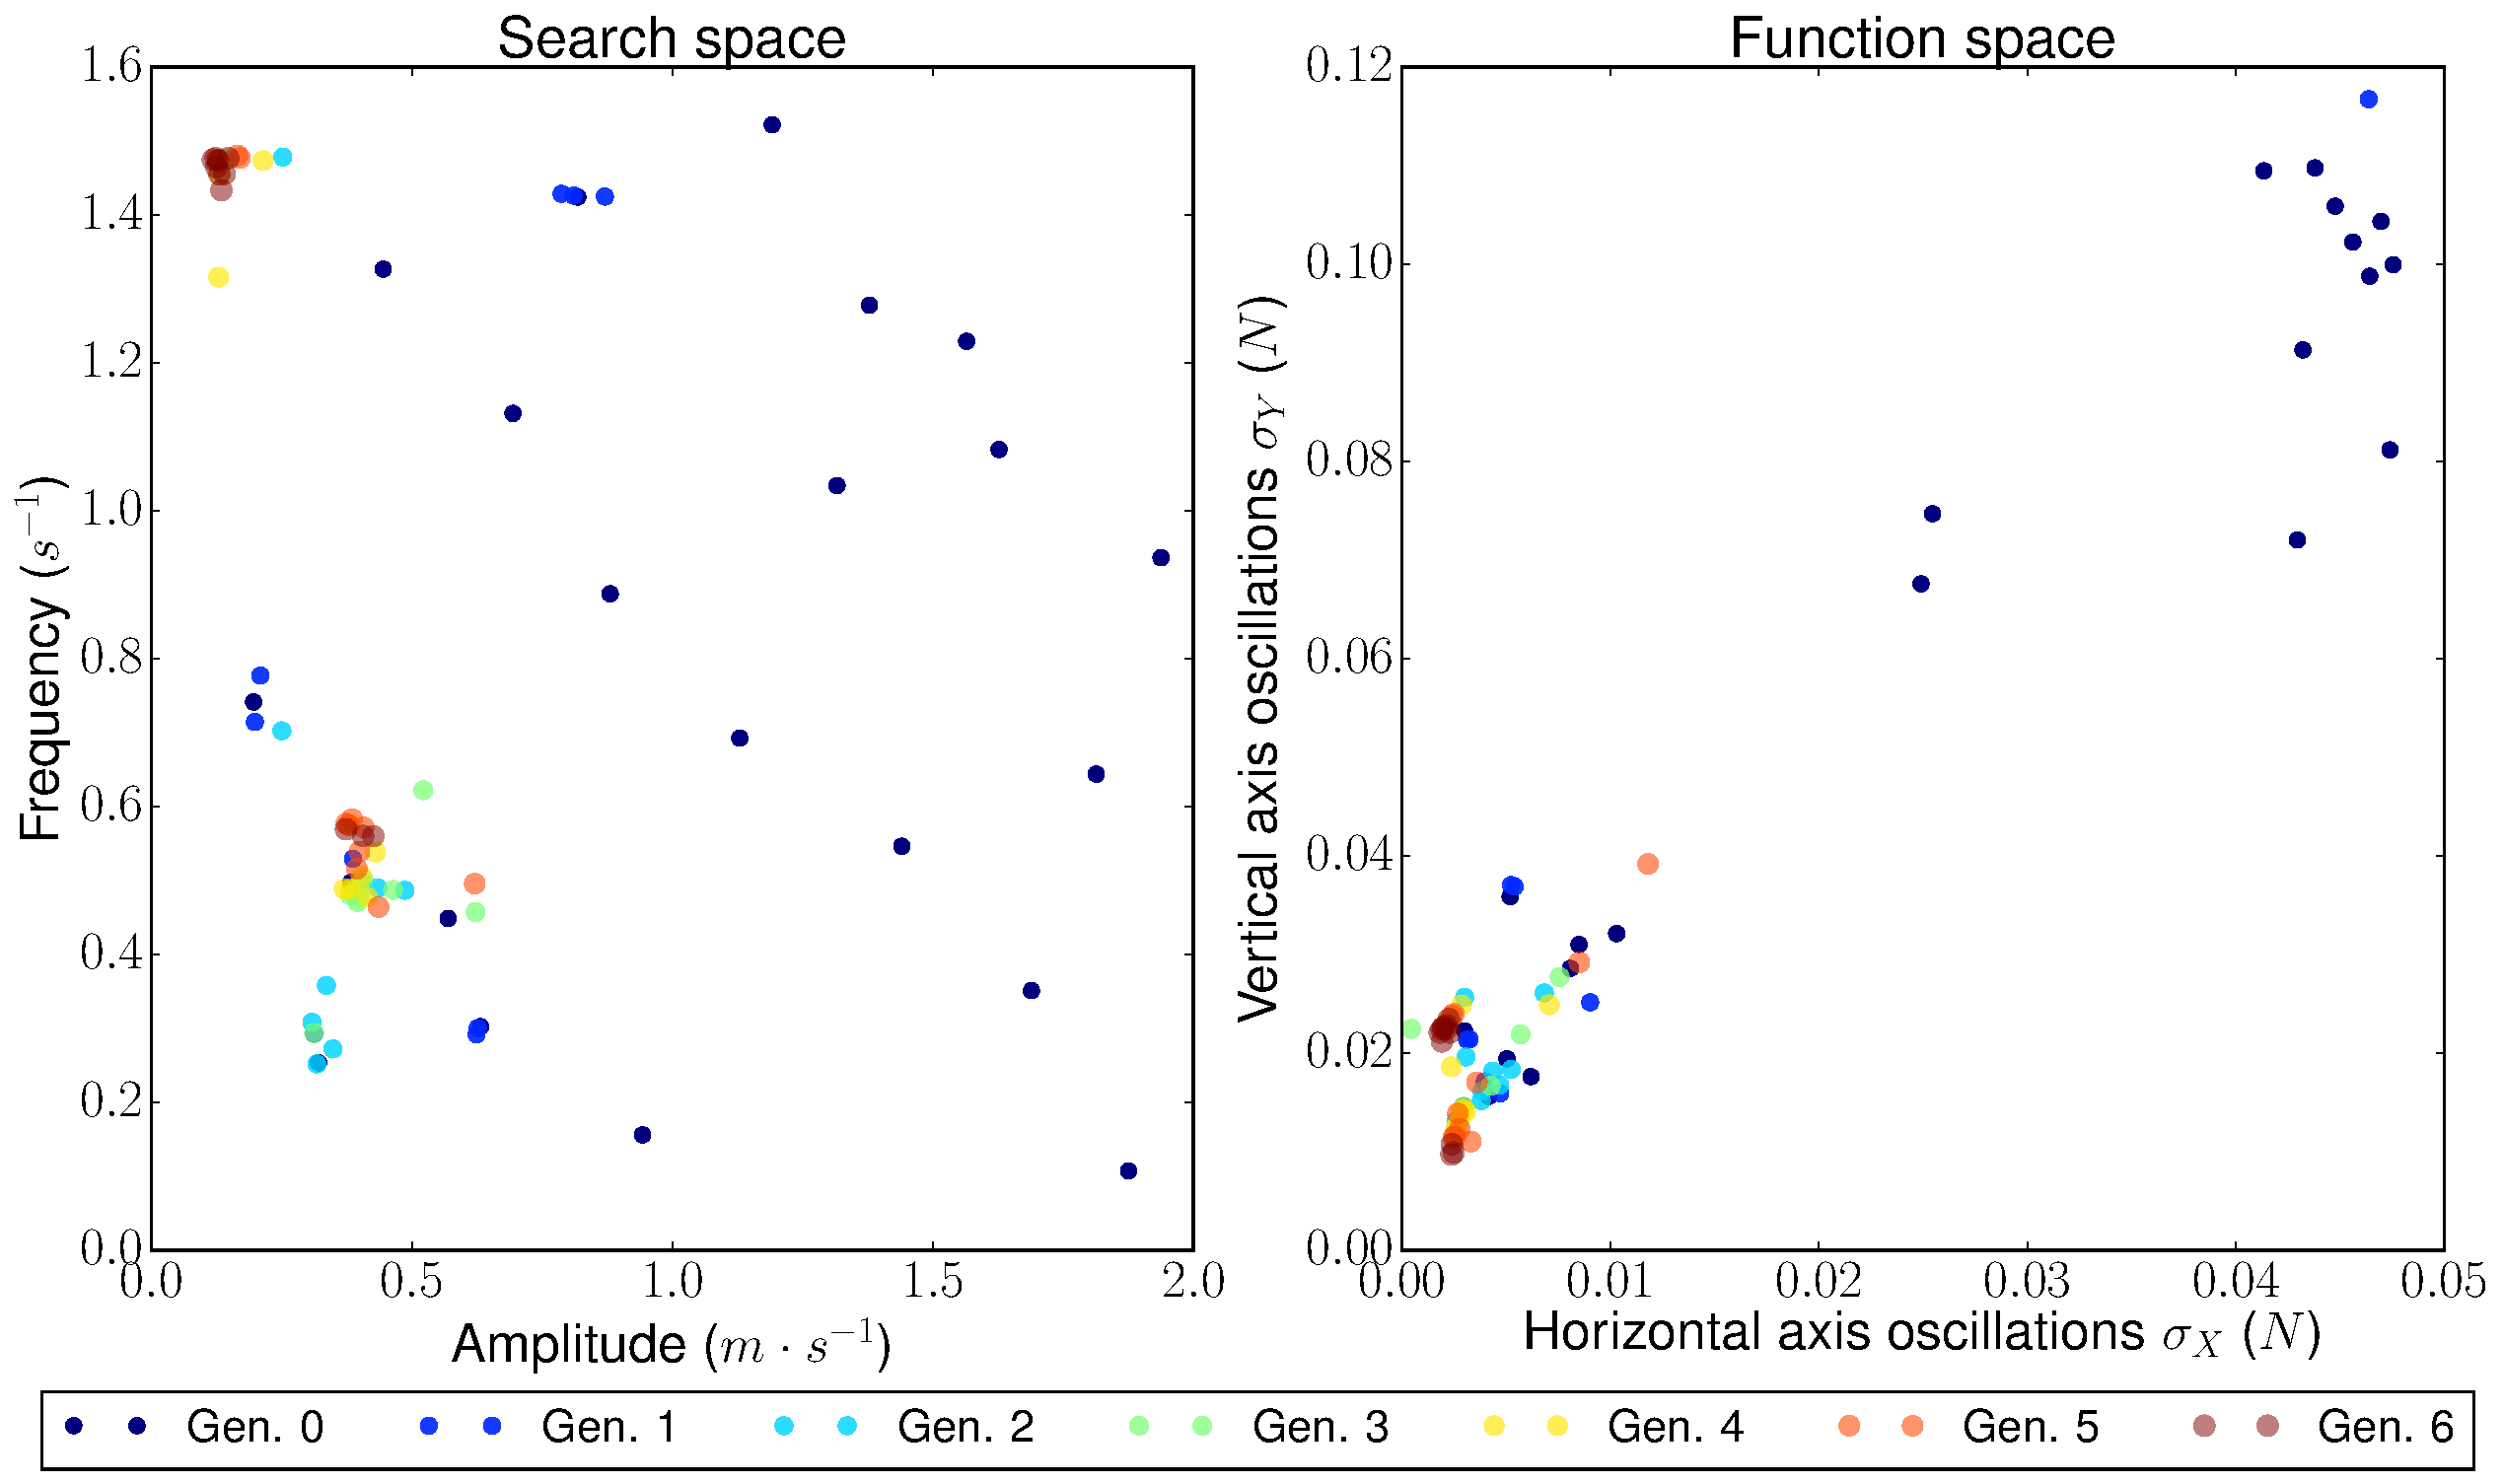
\includegraphics[width=\textwidth, height=0.35\textheight]{Figures/4/gen6.pdf}
        \caption{Evolution of the generations for the cylinder case}
        \label{fig:genForCylinder}
    \end{figure}
    
\begin{figure}[h!]
    \centering
    \begin{subfigure}[t]{0.31\textwidth}
        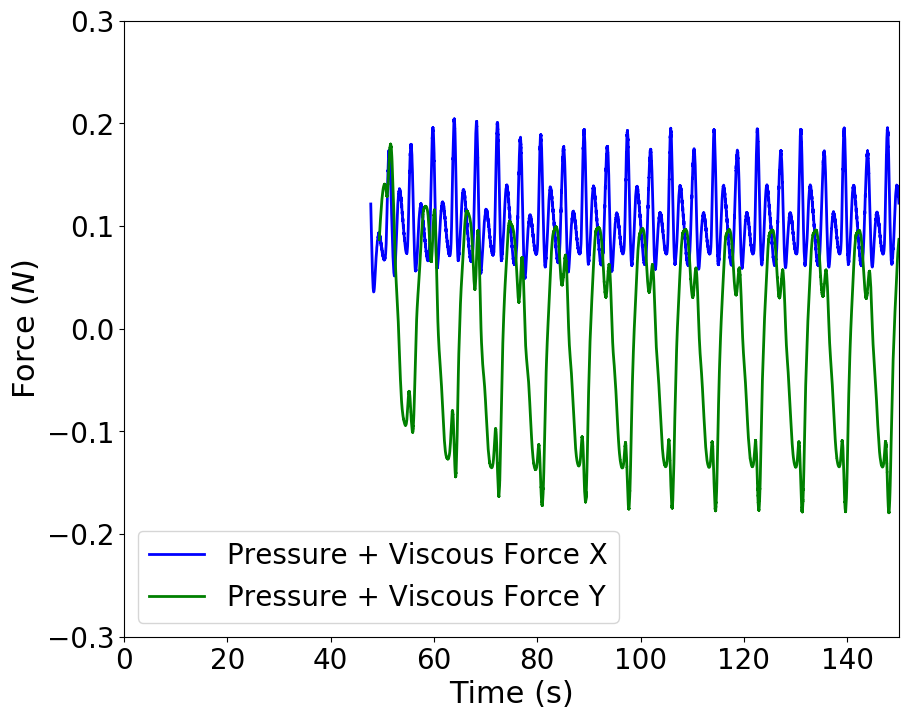
\includegraphics[width=0.95\textwidth, height=0.18\textheight]{Figures/4/OSCg0i37.png}
    \end{subfigure}
    \begin{subfigure}[t]{0.31\textwidth}
        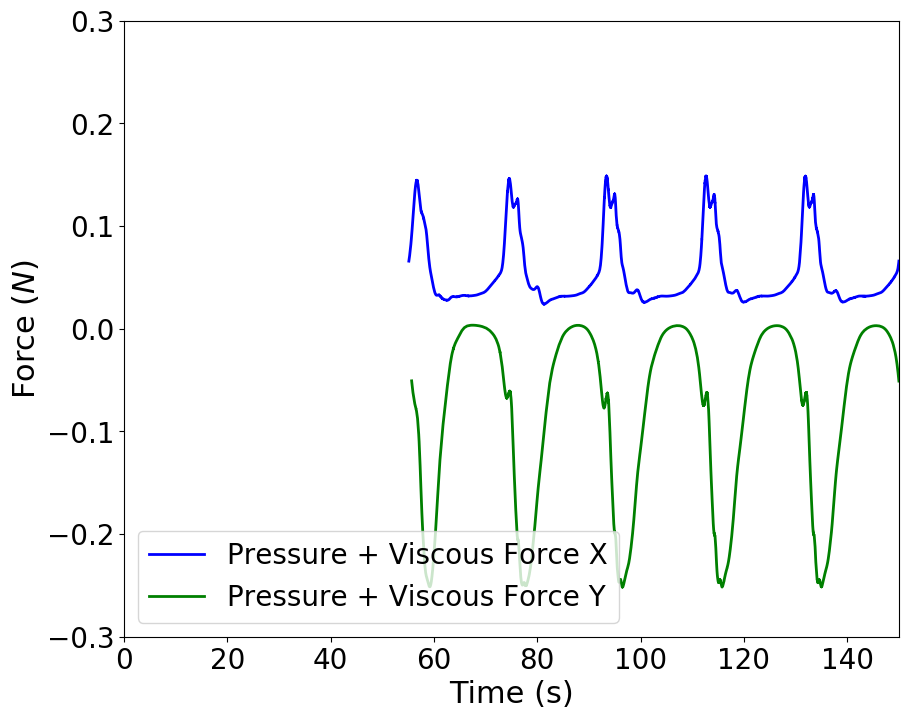
\includegraphics[width=0.95\textwidth, height=0.18\textheight]{Figures/4/OSCg0i38.png}
    \end{subfigure}
    \begin{subfigure}[t]{0.31\textwidth}
        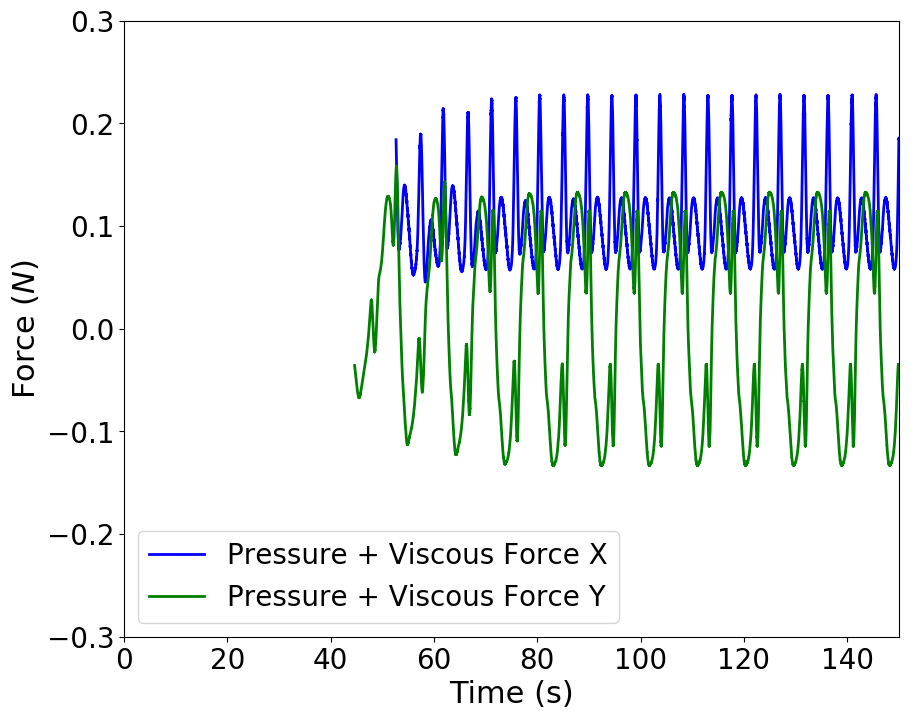
\includegraphics[width=0.95\textwidth, height=0.18\textheight]{Figures/4/OSCg0i45.png}
    \end{subfigure}
    \caption{Sample of the initial generation for the cylinder case}
    \label{fig:initialCyl}
\end{figure}

\begin{figure}[h!]
    \centering
%    \begin{subfigure}[t]{0.15\textwidth}
%    \end{subfigure}
    \begin{subfigure}[t]{0.31\textwidth}
        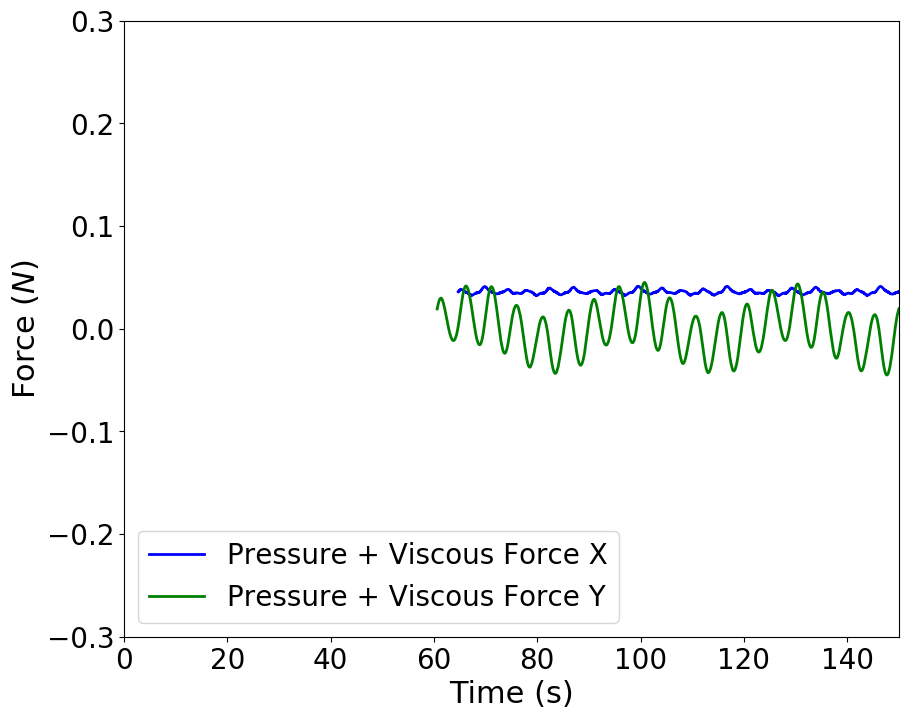
\includegraphics[width=0.95\textwidth, height=0.18\textheight]{Figures/4/OSCg6i6.png}
    \end{subfigure}
    \begin{subfigure}[t]{0.31\textwidth}
        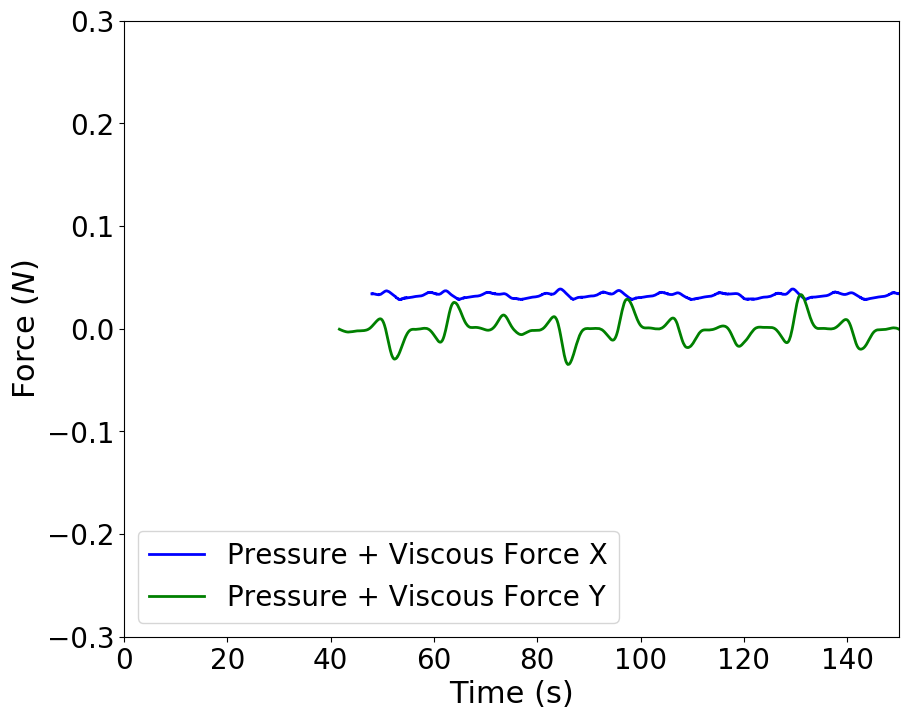
\includegraphics[width=0.95\textwidth, height=0.18\textheight]{Figures/4/OSCg6i3.png}
    \end{subfigure}
    \caption{Sample of the final generation for the cylinder case}
    \label{fig:finalCyl}
\end{figure}

\newpage

\subsubsection*{Inlet of diffuser geometry}

     \begin{figure}[h!]
        \centering
        \small
        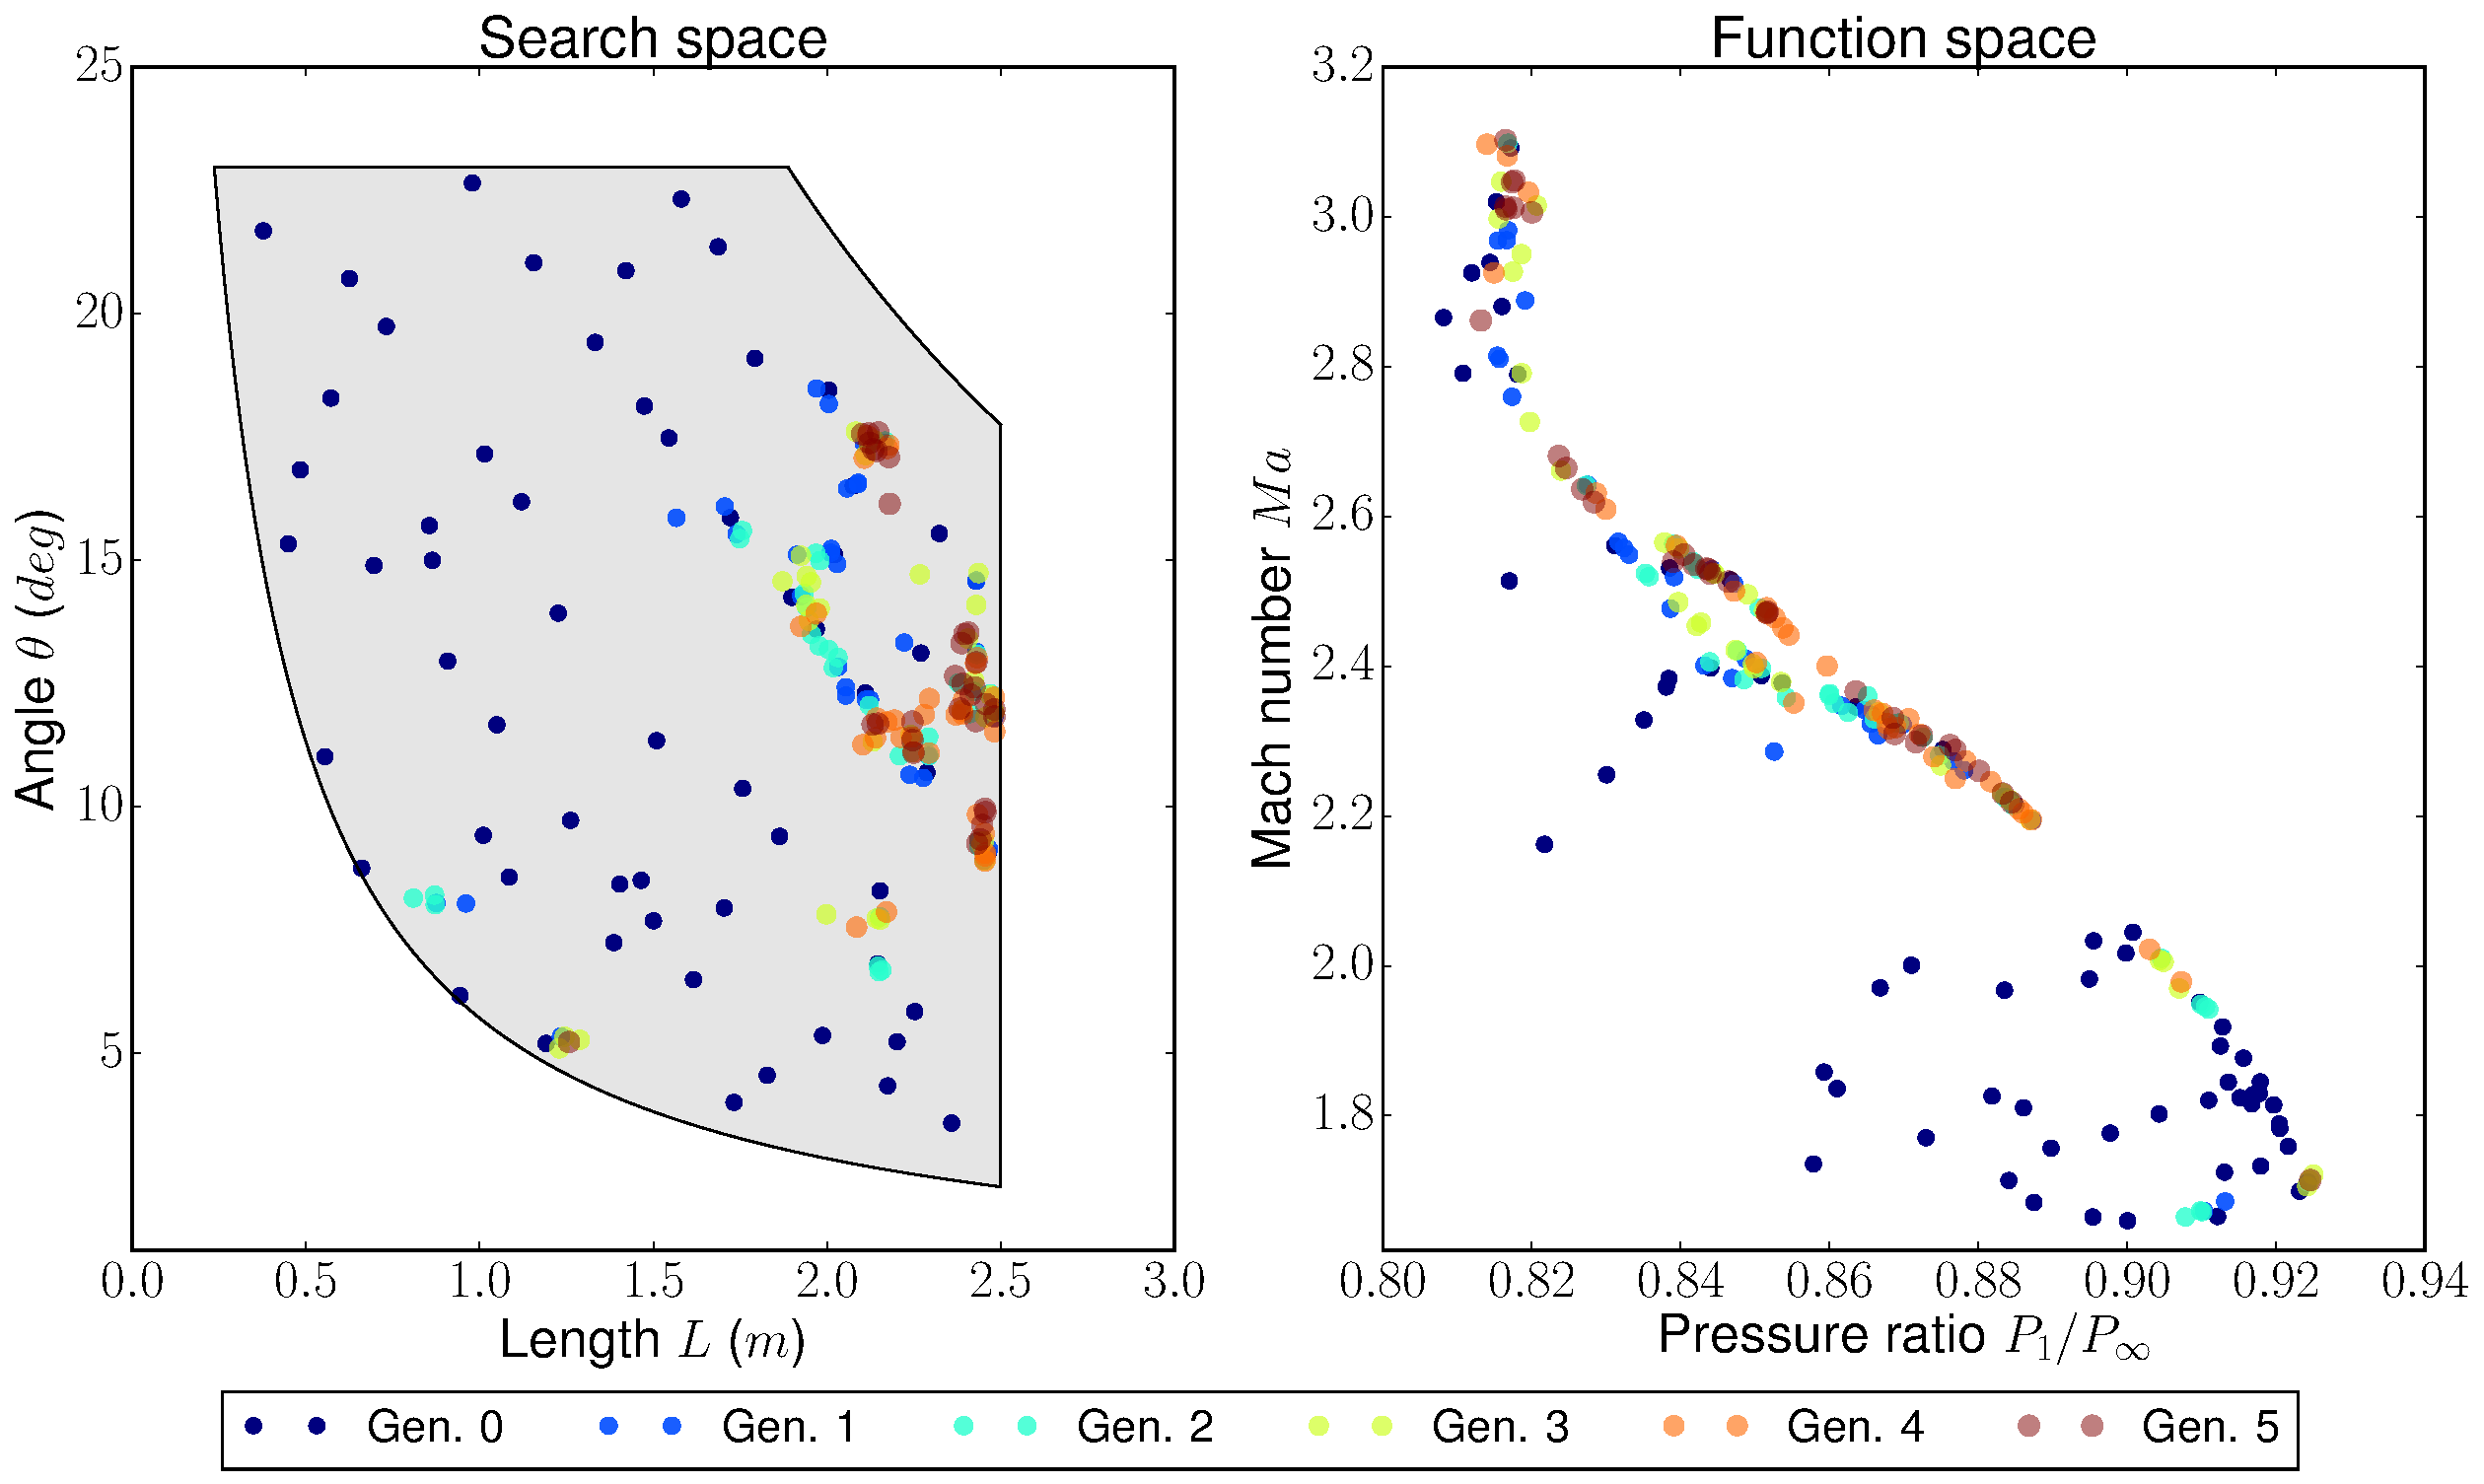
\includegraphics[height=0.35\textheight, width=\textwidth]{Figures/4/gen5.pdf}
        \caption{Evolution of the generations for the diffuser case}
        \label{fig:genForDifusser}
    \end{figure}

\begin{figure}[h!]
    \centering
    \begin{subfigure}[t]{0.31\textwidth}
        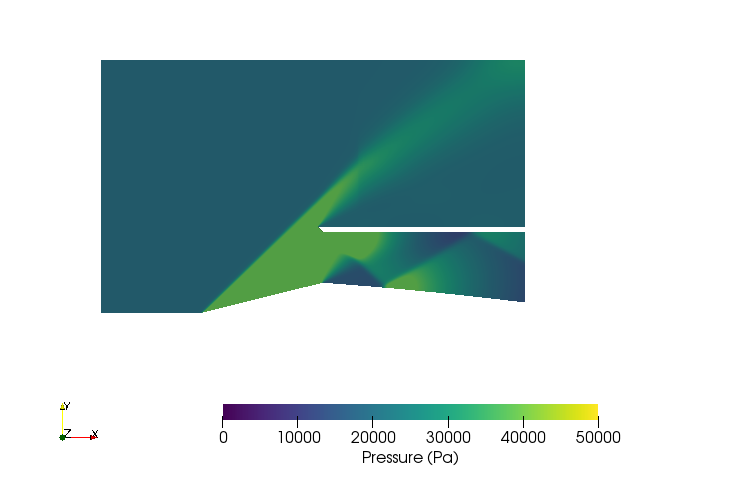
\includegraphics[width=0.95\textwidth, height=0.18\textheight]{Figures/4/SCpg0i3.png}
    \end{subfigure}
    \begin{subfigure}[t]{0.31\textwidth}
        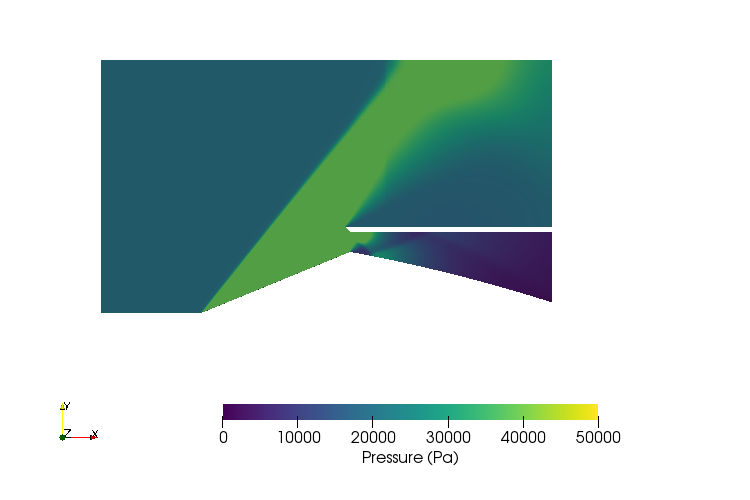
\includegraphics[width=0.95\textwidth, height=0.18\textheight]{Figures/4/SCpg0i9.png}
    \end{subfigure}
    \begin{subfigure}[t]{0.31\textwidth}
        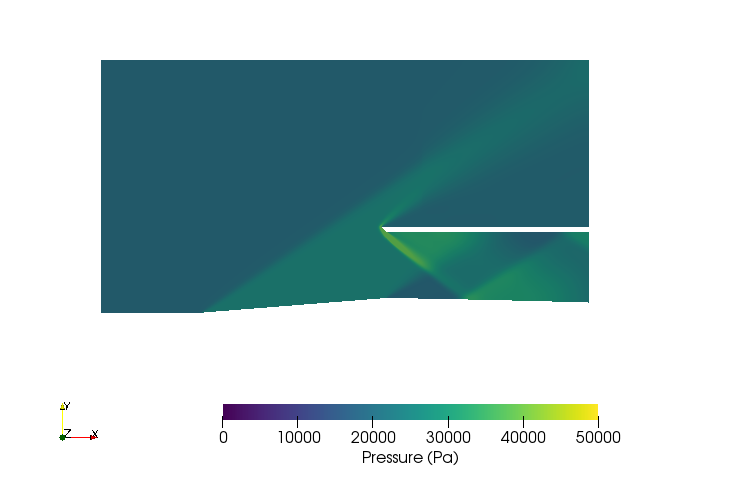
\includegraphics[width=0.95\textwidth, height=0.18\textheight]{Figures/4/SCpg0i46.png}
    \end{subfigure}
    \caption{Sample of the initial generation for the diffuser case}
            \label{fig:initialDif}
\end{figure}

\begin{figure}[h!]
    \centering
    \begin{subfigure}[t]{0.31\textwidth}
        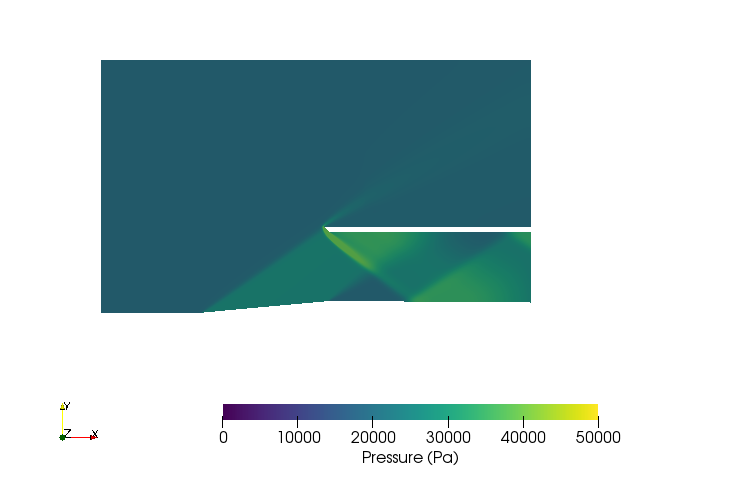
\includegraphics[width=0.95\textwidth, height=0.18\textheight]{Figures/4/SCpg5i9.png}
    \end{subfigure}
    \begin{subfigure}[t]{0.31\textwidth}
        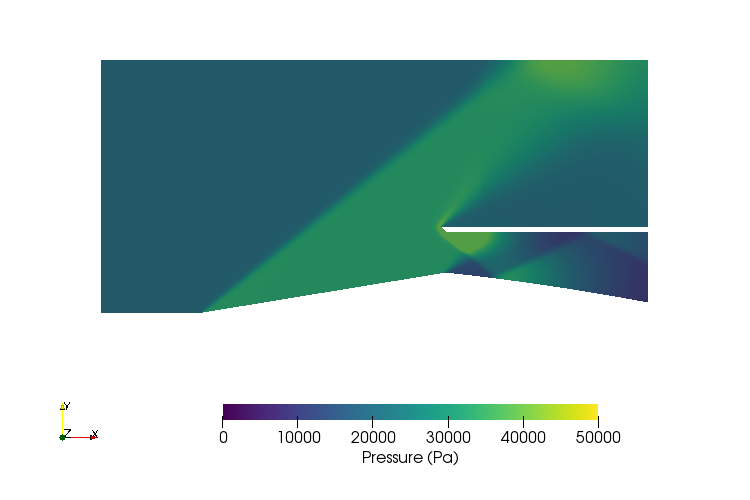
\includegraphics[width=0.95\textwidth, height=0.18\textheight]{Figures/4/SCpg5i14.png}
    \end{subfigure}
    \begin{subfigure}[t]{0.31\textwidth}
        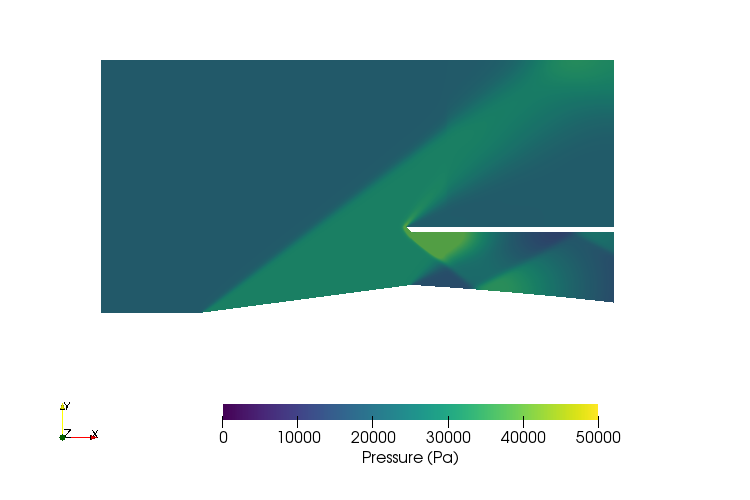
\includegraphics[width=0.95\textwidth, height=0.18\textheight]{Figures/4/SCpg5i18.png}
    \end{subfigure}
    \caption{Sample of the final generation for the diffuser case}
    \label{fig:finalDif}
\end{figure}


\newpage

\subsubsection*{Airfoil design: lift maximization and drag minimization}

     \begin{figure}[h!]
        \centering
        \small
        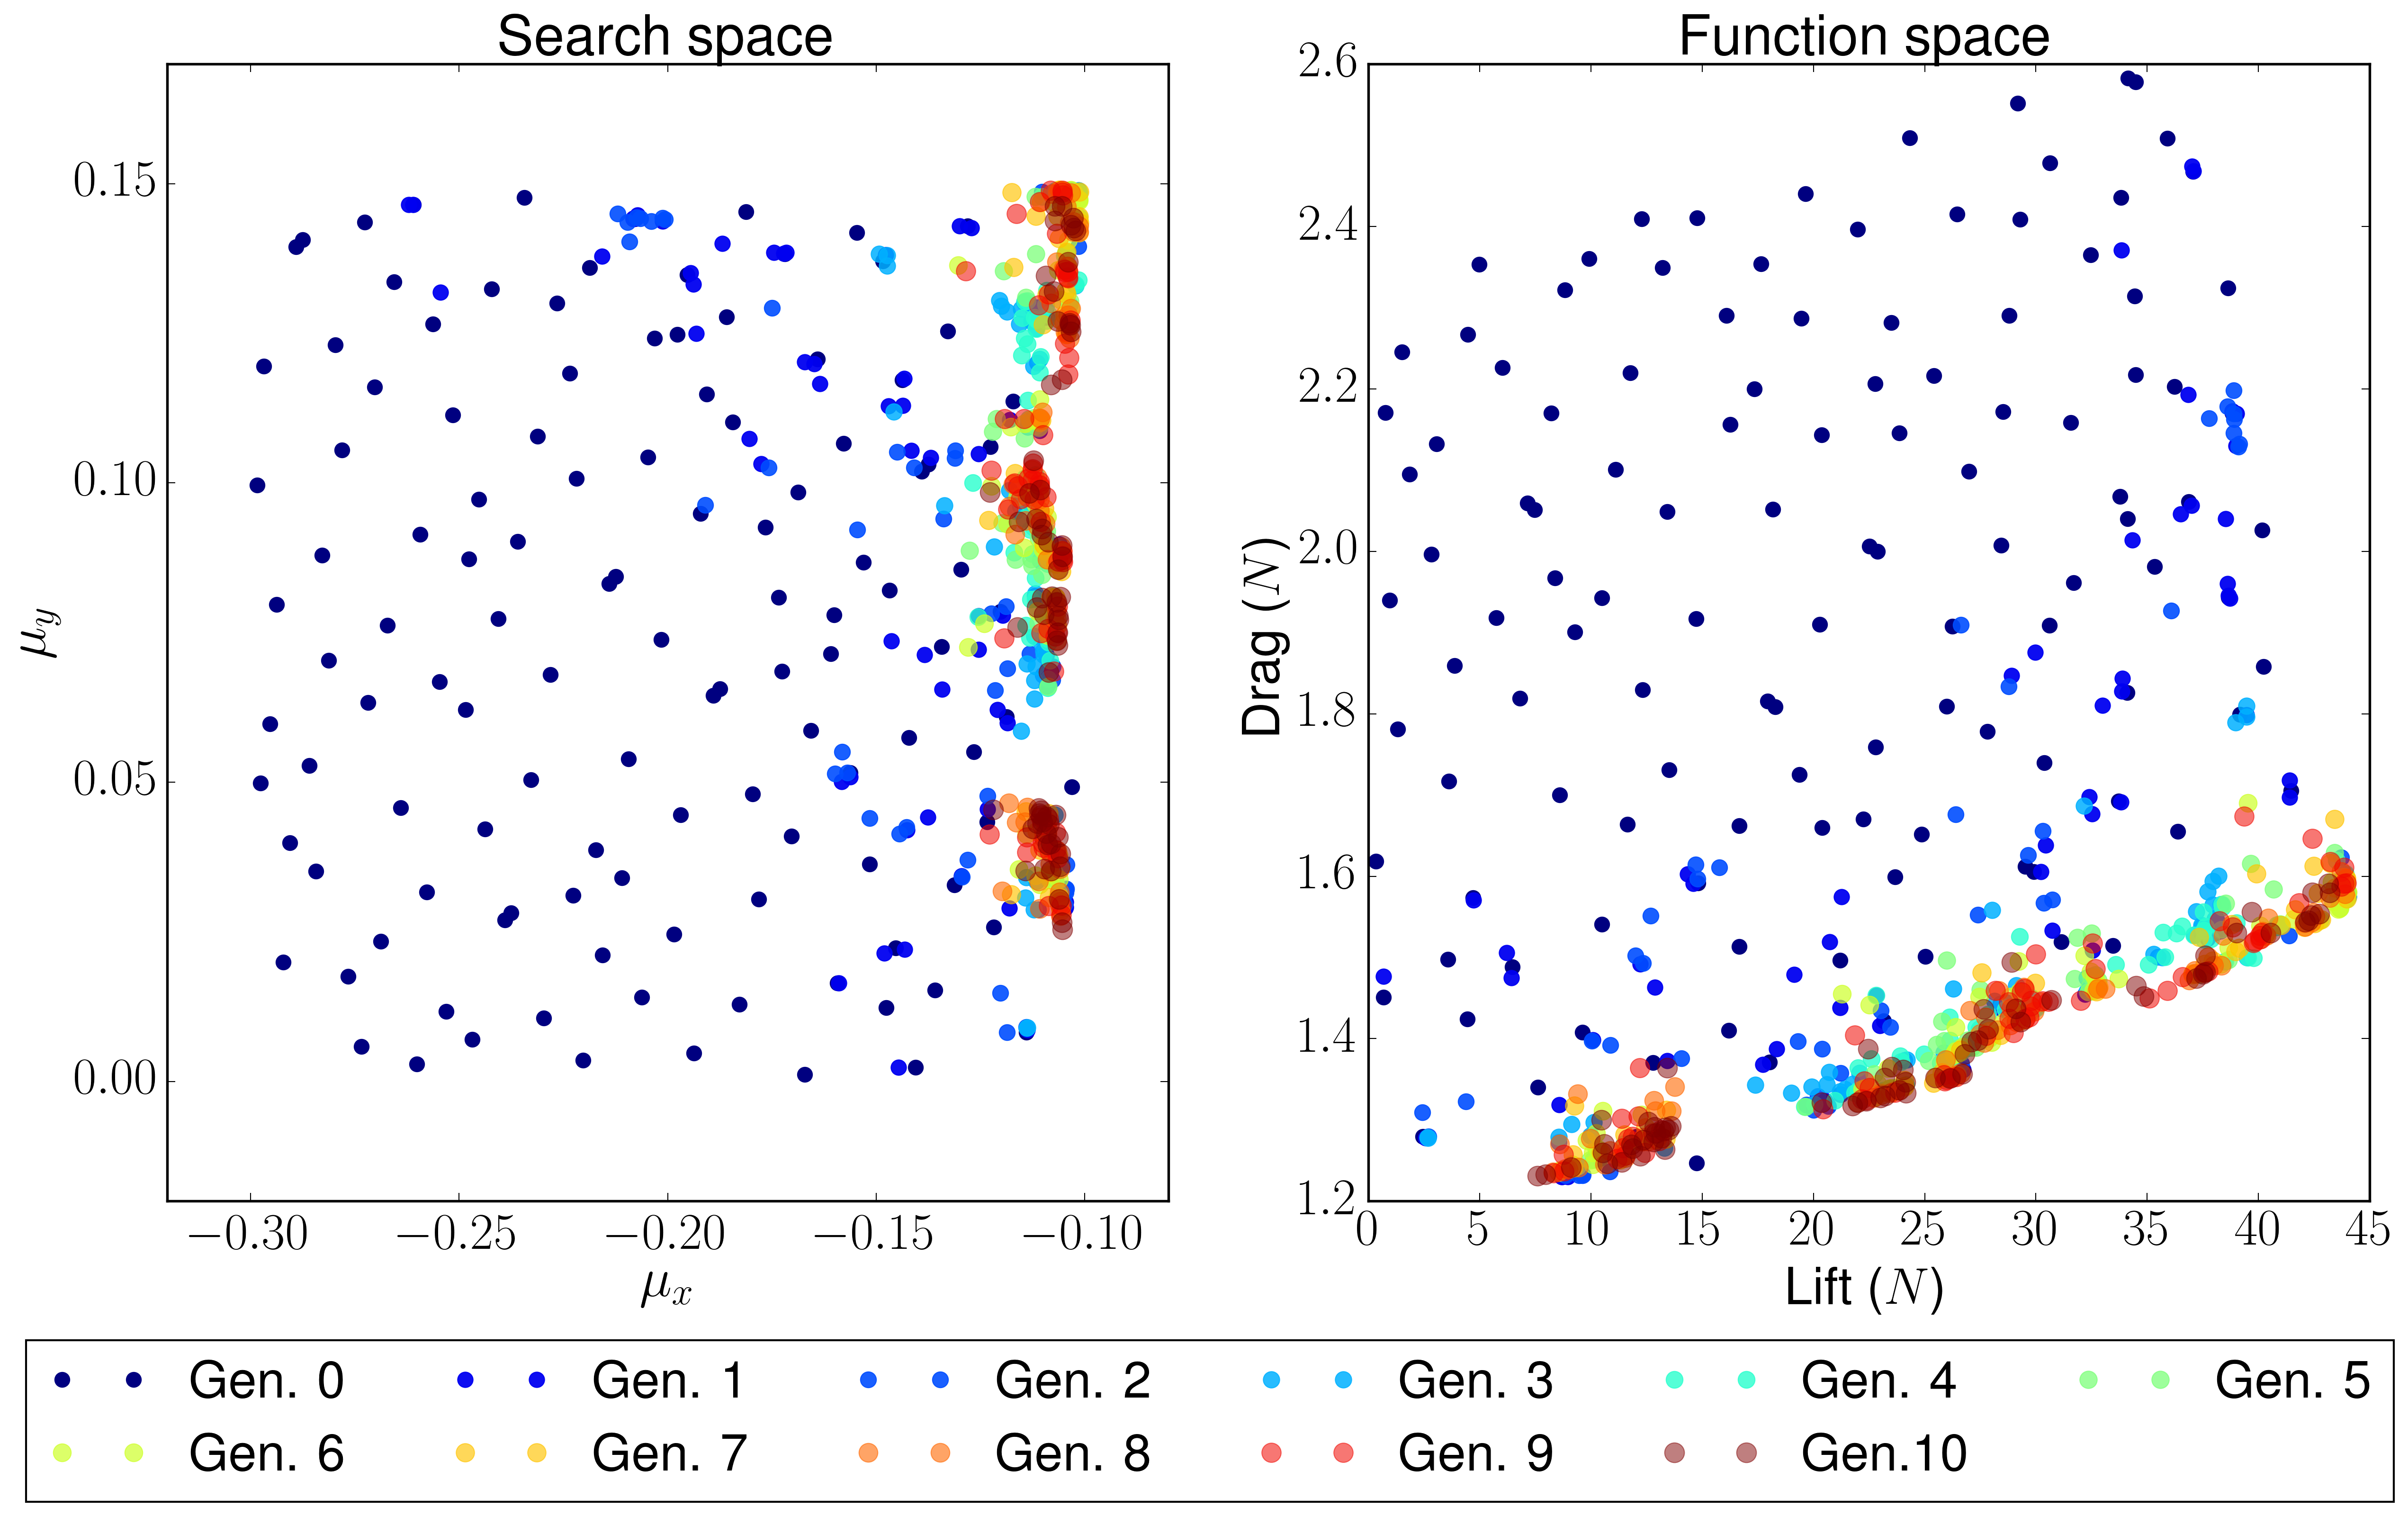
\includegraphics[width=\textwidth, height=0.4\textheight]{Figures/4/cLcDgen10.png}
        \caption{Evolution of the generations for the airfoil case I}
        \label{fig:genForCLCD}
    \end{figure}


\begin{figure}[h!]
    \centering
    \begin{subfigure}[t]{0.31\textwidth}
        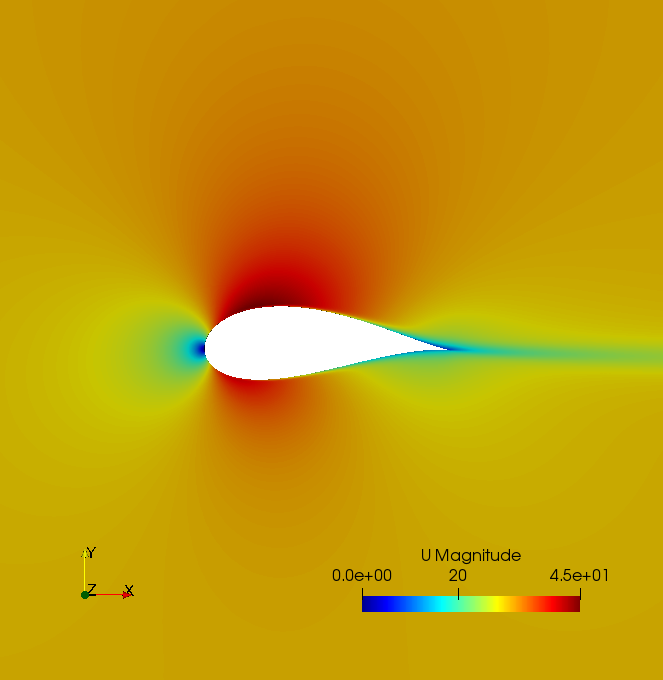
\includegraphics[width=0.95\textwidth, height=0.17\textheight]{Figures/4/g0i116.png}
    \end{subfigure}
    \begin{subfigure}[t]{0.31\textwidth}
        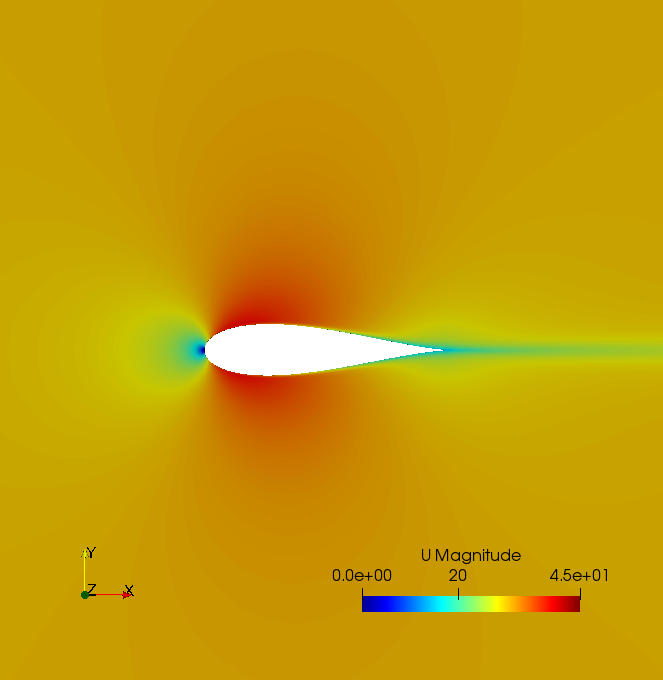
\includegraphics[width=0.95\textwidth, height=0.17\textheight]{Figures/4/g0i19.png}
    \end{subfigure}
    \begin{subfigure}[t]{0.31\textwidth}
        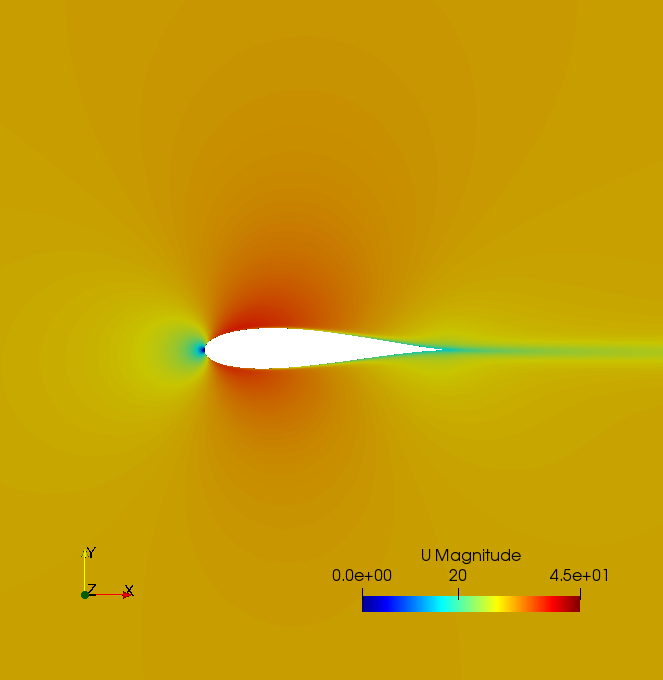
\includegraphics[width=0.95\textwidth, height=0.17\textheight]{Figures/4/g0i55.png}
    \end{subfigure}
    \caption{Sample of the initial generation for the airfoil case I}
    \label{fig:initialCLCD}
\end{figure}

\begin{figure}[h!]
    \centering
    \begin{subfigure}[t]{0.31\textwidth}
        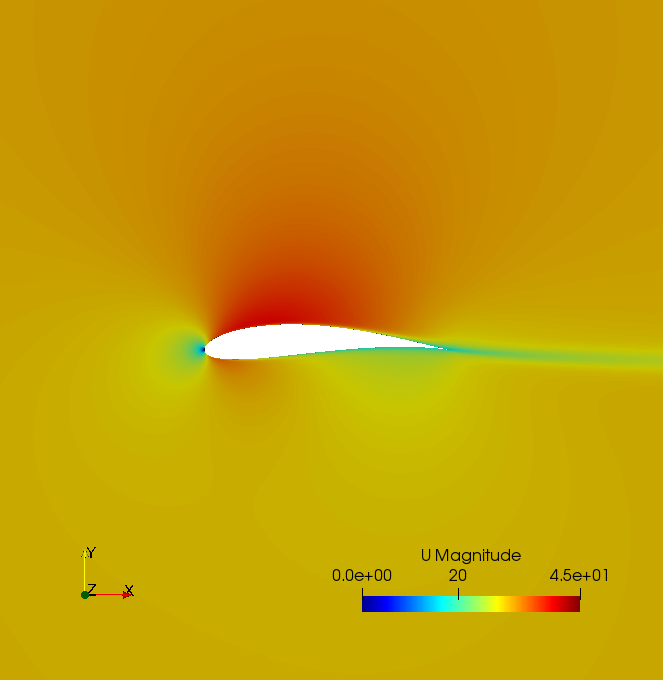
\includegraphics[width=0.95\textwidth, height=0.17\textheight]{Figures/4/g10i14.png}
    \end{subfigure}
    \begin{subfigure}[t]{0.31\textwidth}
        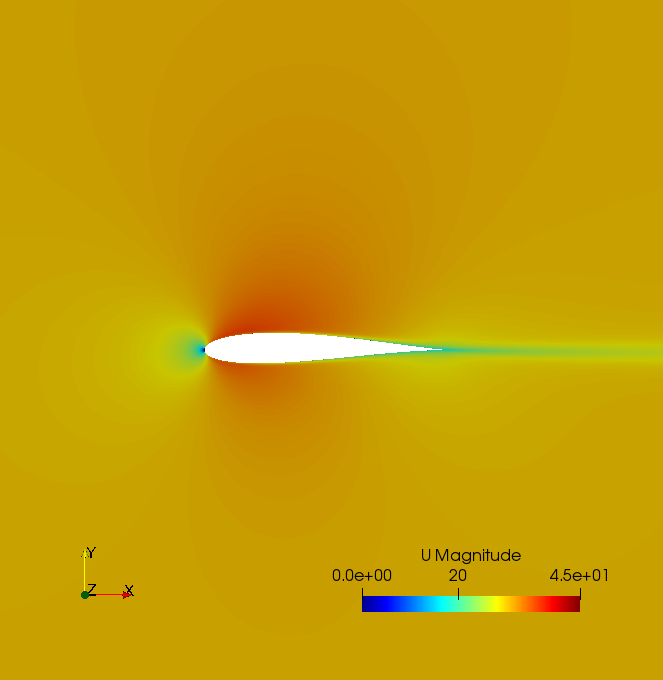
\includegraphics[width=0.95\textwidth, height=0.17\textheight]{Figures/4/g10i35.png}
    \end{subfigure}
    \begin{subfigure}[t]{0.31\textwidth}
        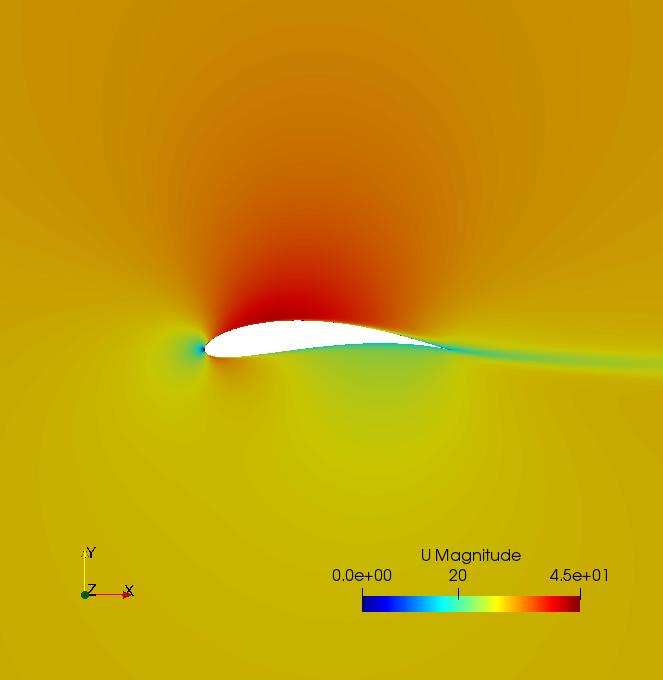
\includegraphics[width=0.95\textwidth, height=0.17\textheight]{Figures/4/g10i55.png}
    \end{subfigure}
    \caption{Sample of the final generation for the airfoil case I}
    \label{fig:finalCLCD}
\end{figure}

    
\subsubsection*{Airfoil design: lift-to-drag ratio and area maximization}

     \begin{figure}[h!]
        \centering
        \small
        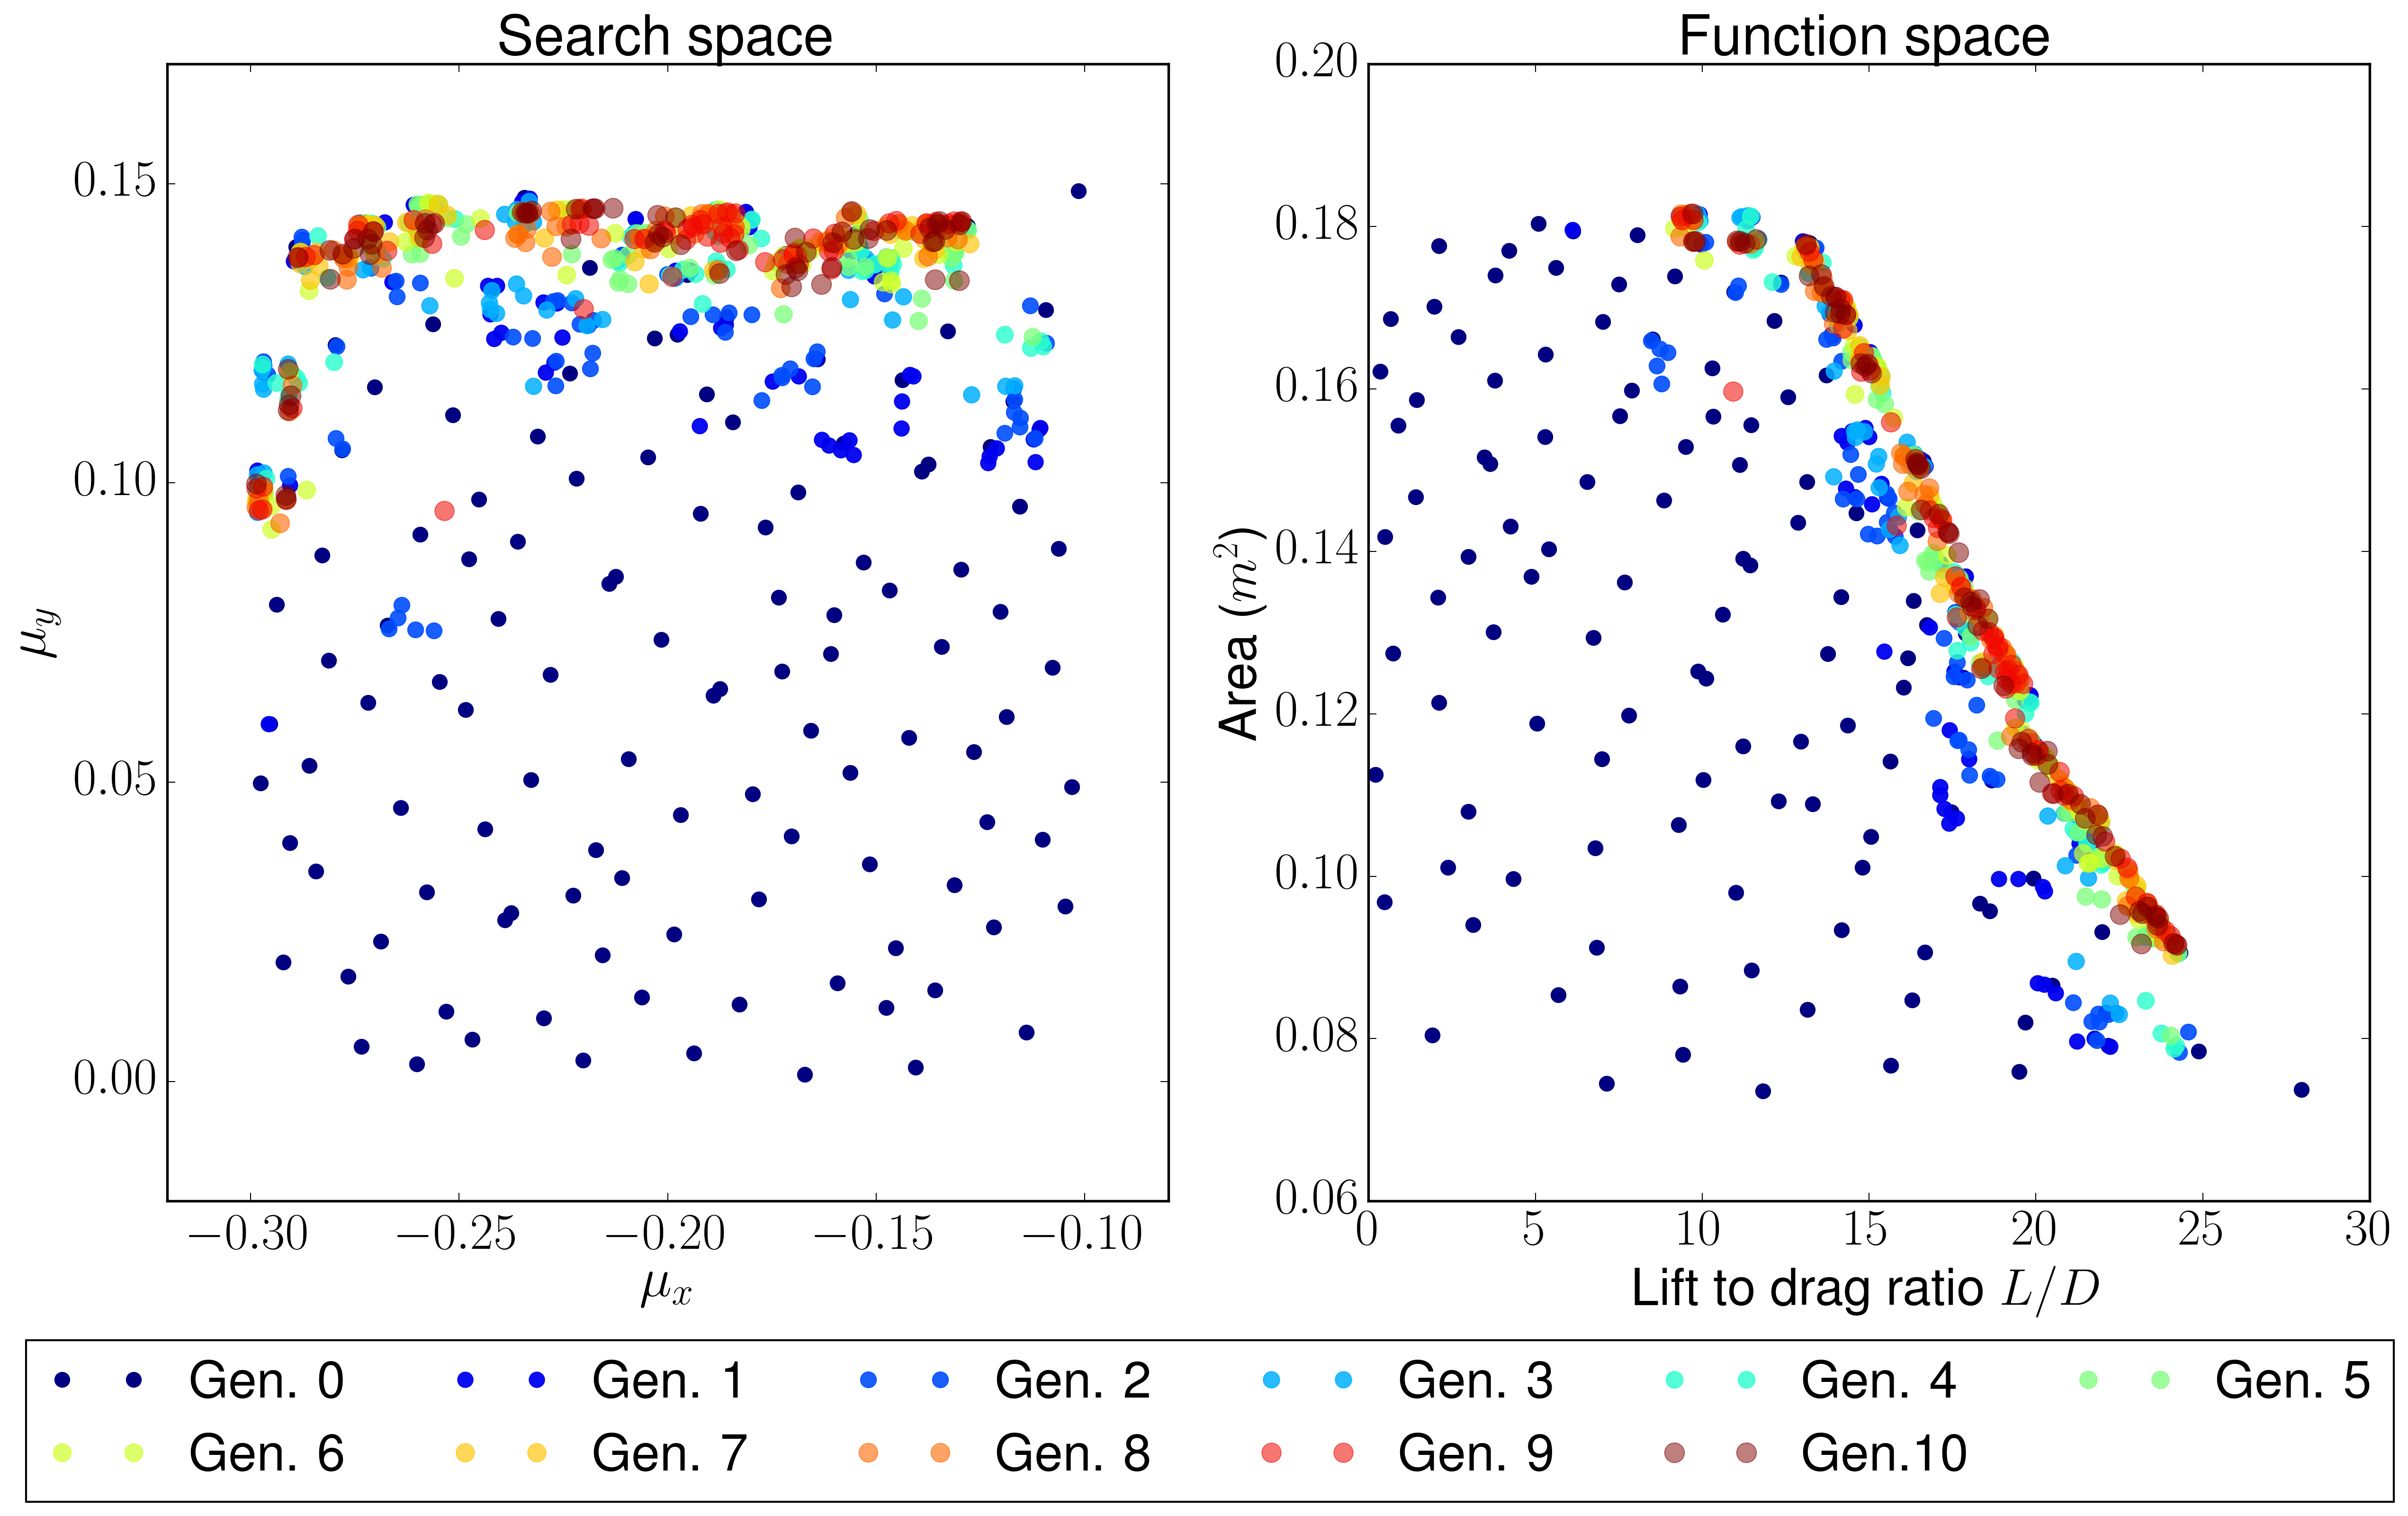
\includegraphics[width=\textwidth, height=0.4\textheight]{Figures/4/LDgen10.png}
        \caption{Evolution of the generations for the airfoil case II}
        \label{fig:genForLD}
    \end{figure}
    
    
    \begin{figure}[h!]
    \centering
    \begin{subfigure}[t]{0.31\textwidth}
        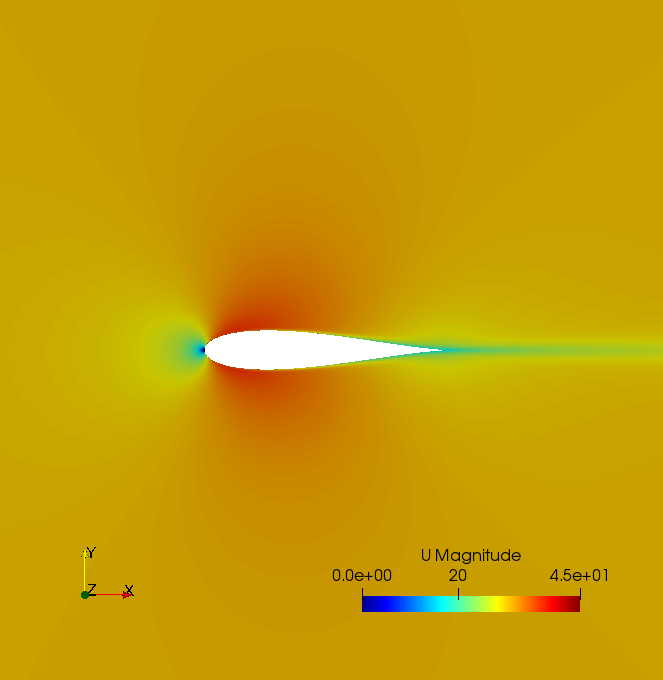
\includegraphics[width=0.95\textwidth, height=0.17\textheight]{Figures/4/LDAg0i23.png}
    \end{subfigure}
    \begin{subfigure}[t]{0.31\textwidth}
        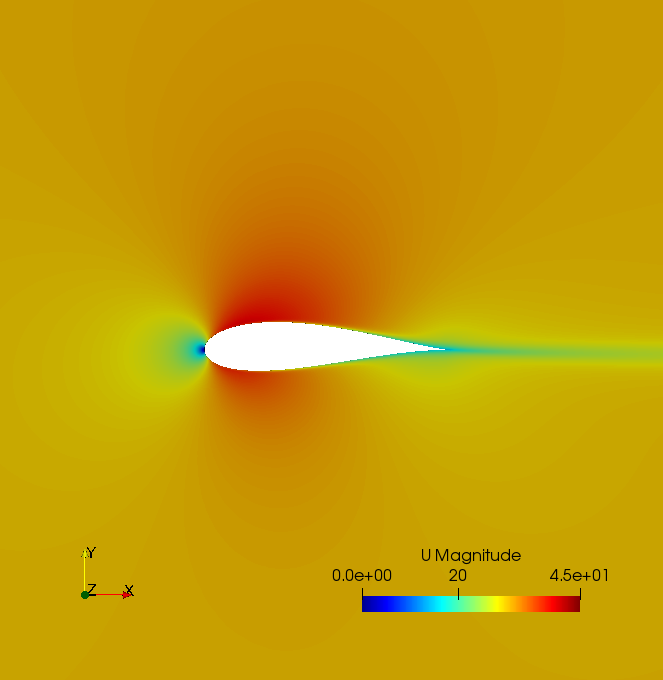
\includegraphics[width=0.95\textwidth, height=0.17\textheight]{Figures/4/LDAg0i99.png}
    \end{subfigure}
    \begin{subfigure}[t]{0.31\textwidth}
        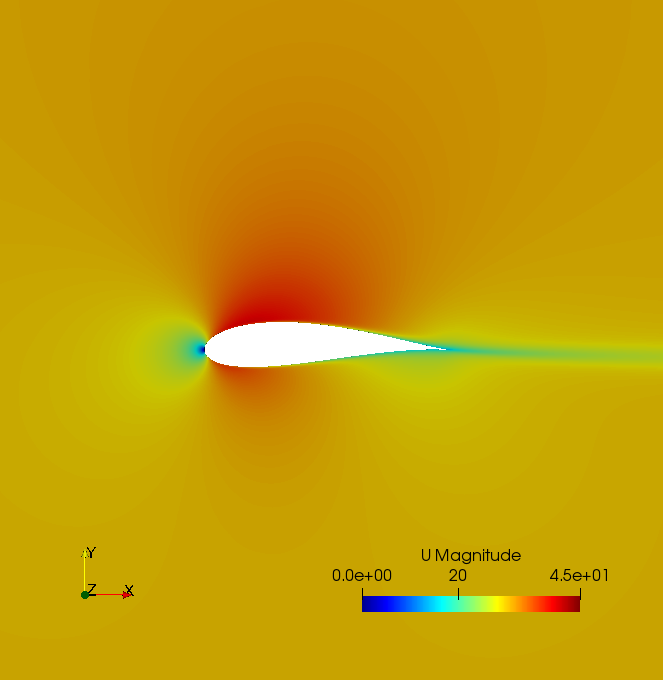
\includegraphics[width=0.95\textwidth, height=0.17\textheight]{Figures/4/LDAg0i107.png}
    \end{subfigure}
    \caption{Sample of the initial generation for the airfoil case II}
    \label{fig:initialLD}
\end{figure}

\begin{figure}[h!]
    \centering
    \begin{subfigure}[t]{0.31\textwidth}
        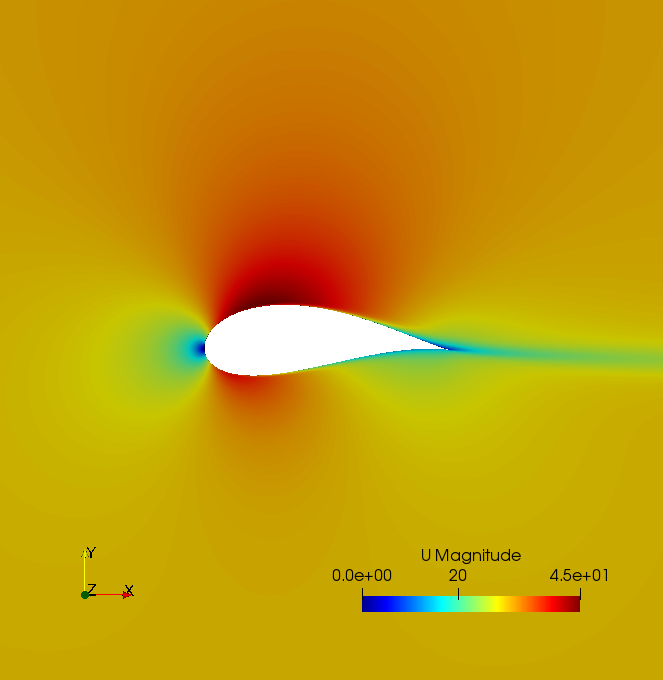
\includegraphics[width=0.95\textwidth, height=0.17\textheight]{Figures/4/LDAg10i11.png}
    \end{subfigure}
    \begin{subfigure}[t]{0.31\textwidth}
        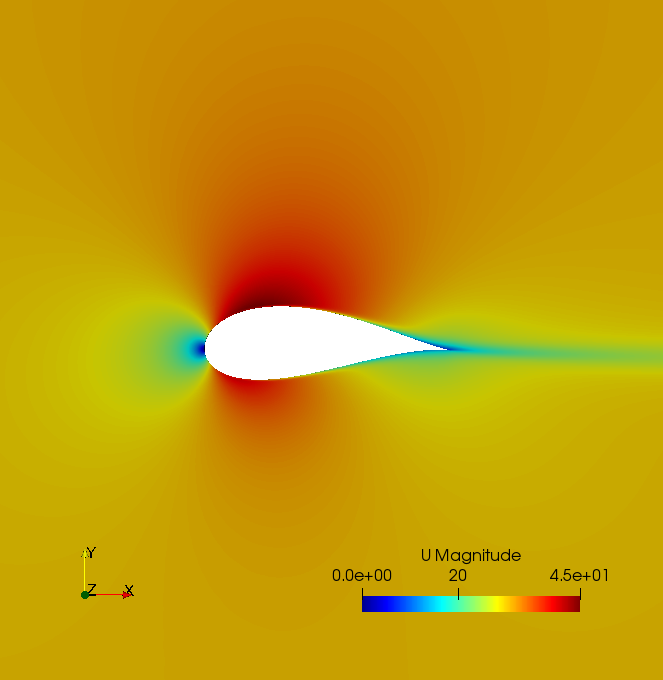
\includegraphics[width=0.95\textwidth, height=0.17\textheight]{Figures/4/LDAg10i47.png}
    \end{subfigure}
    \begin{subfigure}[t]{0.31\textwidth}
        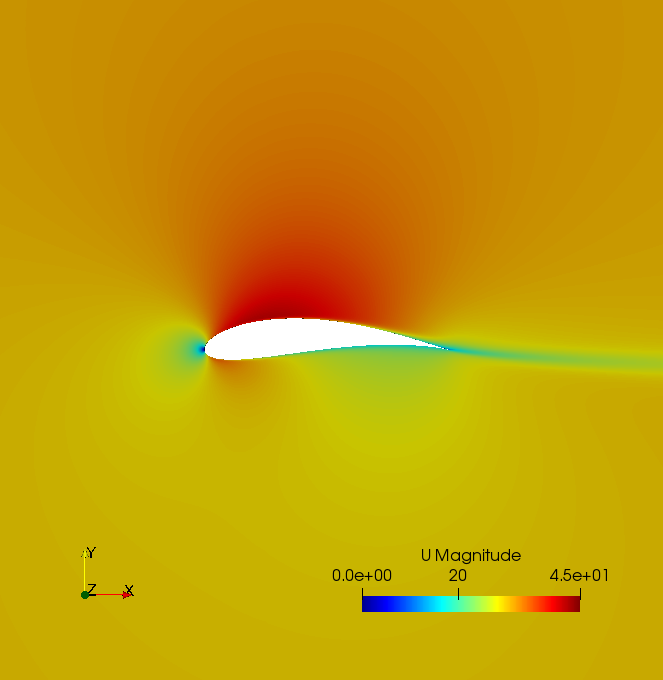
\includegraphics[width=0.95\textwidth, height=0.17\textheight]{Figures/4/LDAg10i53.png}
    \end{subfigure}
    \caption{Sample of the final generation for the airfoil case II}
    \label{fig:finalLD}
\end{figure}
